\section{Auswertung}

\subsection{Kennlinienschar durch Variation der Heizleistung}


\begin{flushleft}
    Gemessen wurden fünf Kennlinien durch Variation der Heizleistung.
    Die Messwerte der fünf Kennlinien befinden sich in Tabelle \ref{Tabelle1}.
\end{flushleft} 

\begin{table}[H]
    \centering
    \caption{Die Messwerte der fünf Kennlinien} 
    \label{Tabelle1}
    \begin{tabular} {c  c  c  c  c  c  c}
        \toprule
        { } &
        {Kennlinie 1} &
        {Kennlinie 2} &
        {Kennlinie 3} &
        {Kennlinie 4} &
        {Kennlinie 5} &
        {Kennlinie 6} \\
        \midrule
        {$ \text{U} \mathbin{/} \unit{\volt} $} & 
        {$ \text{I} \mathbin{/} \unit{\milli\ampere} $} &
        {$ \text{I} \mathbin{/} \unit{\milli\ampere} $} &
        {$ \text{I} \mathbin{/} \unit{\milli\ampere} $} &
        {$ \text{I} \mathbin{/} \unit{\milli\ampere} $} &
        {$ \text{I} \mathbin{/} \unit{\milli\ampere} $} &
        {$ \text{I} \mathbin{/} \unit{\milli\ampere} $} \\
        \hline
        10  & 0,05  & 0,055 & 0,084 & 0,068 & 0,109 & 0,121 \\
        15  & -     & 0,103 & 0,150 & 0,134 & 0,192 & 0,208 \\
        20  & 0,104 & 0,154 & 0,232 & 0,222 & 0,282 & 0,300 \\
        25  & -     & 0,197 & 0,310 & 0,309 & 0,398 & 0,402 \\
        30  & 0,123 & 0,227 & 0,385 & 0,420 & 0,516 & 0,516 \\
        40  & 0,129 & 0,256 & 0,525 & 0,602 & 0,744 & 0,750 \\
        50  & 0,130 & 0,268 & 0,628 & 0,753 & 0,988 & 1,007 \\
        60  & 0,131 & 0,272 & 0,727 & 0,874 & 1,209 & 1,200 \\
        70  & 0,132 & 0,275 & 0,731 & 0,945 & 1,414 & 1,604 \\
        80  & 0,133 & 0,277 & 0,738 & 0,995 & 1,602 & 1,953 \\
        90  & -     & -     &  -    & 1,006 & 1,714 & -     \\
        100 & -     & -     &  -    & 1,012 & -     & -     \\
        \bottomrule
    \end{tabular} 
\end{table}

\begin{flushleft}
    Aus den Messwerten werden Graphen erstellt. 
    Dabei bildet sich eine Asymptote und an der wird der Sättigungstrom $\text{I}_{\text{S}}$ wie in Abbildung \ref{Abbildung2}.
    Der Sättigungsstrom wird in Tabelle \ref{Tabelle2}.
\end{flushleft}

\begin{figure}[H]
    \centering
    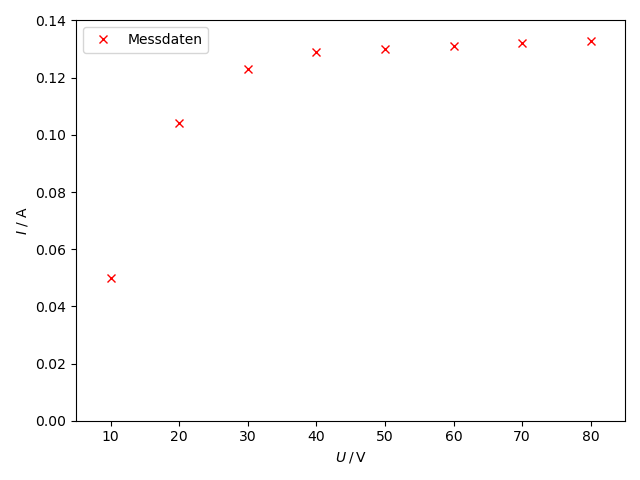
\includegraphics[height=80mm]{bilder/K1.png}
    \caption{Kennlinie 1 mit $\text{I}_{\text{Heiz}} = 2,0\,\unit{\ampere} $. \label{Abbildung6} }
\end{figure}

\begin{figure}[H]
    \centering
    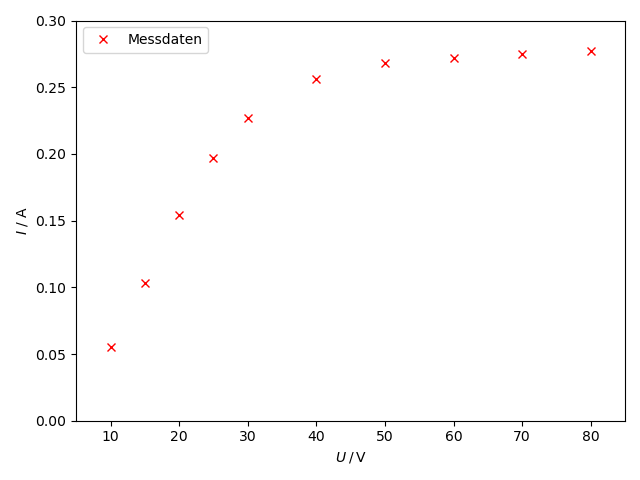
\includegraphics[height=80mm]{bilder/K2.png}
    \caption{Kennlinie 2 mit $\text{I}_{\text{Heiz}} = 2,1\,\unit{\ampere} $.\label{Abbildung7} }
\end{figure}

\begin{figure}[H]
    \centering
    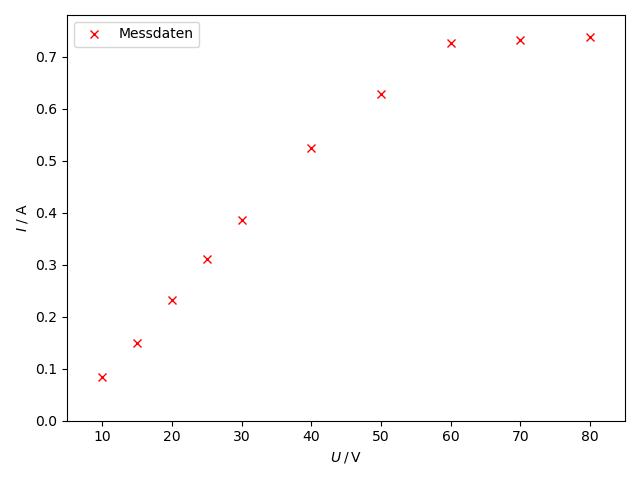
\includegraphics[height=80mm]{bilder/K3.png}
    \caption{Kennlinie 3 mit $\text{I}_{\text{Heiz}} = 2,2\,\unit{\ampere} $.\label{Abbildung8} }
\end{figure}

\begin{figure}[H]
    \centering
    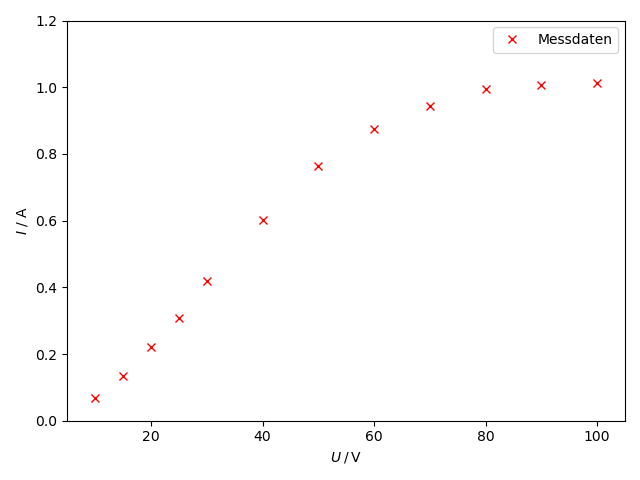
\includegraphics[height=80mm]{bilder/K4.png}
    \caption{Kennlinie 4 mit $\text{I}_{\text{Heiz}} = 2,3\,\unit{\ampere} $.\label{Abbildung9} }
\end{figure}

\begin{figure}[H]
    \centering
    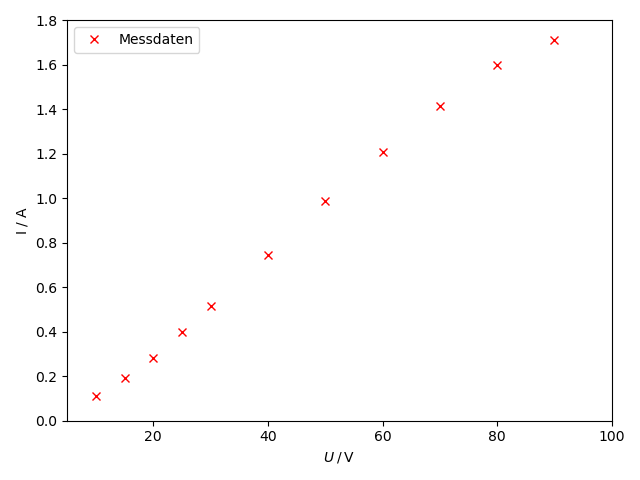
\includegraphics[height=80mm]{bilder/K5.png}
    \caption{Kennlinie 5 mit $\text{I}_{\text{Heiz}} = 2,4\,\unit{\ampere} $.\label{Abbildung10} }
\end{figure}

\begin{figure}[H]
    \centering
    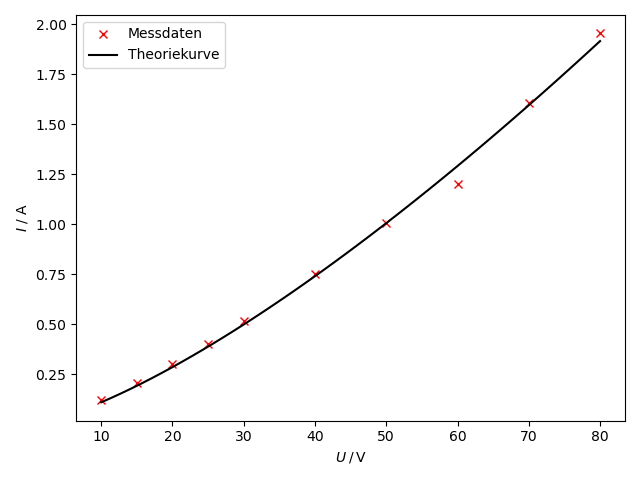
\includegraphics[height=80mm]{bilder/K6.png}
    \caption{Kennlinie 6 mit $\text{I}_{\text{Heiz}} = 2,5\,\unit{\ampere} $.\label{Abbildung11} }
\end{figure}


\begin{table}[H]     % Tabelle mit einer Spalte
    \centering
    \caption{Der Sättigungsstrom}
    \label{Tabelle2}
    \begin{tabular} {c c}
        \toprule
        {Kennlinie} &
        {$\text{I}_{\text{S}} \mathbin{/} \unit{\milli\ampere} $} \\
        \midrule
        1 & 0,1338 \\
        2 & 0,2821 \\
        3 & 0,750 \\
        4 & 1,014 \\
        5 & 1,720 \\
        6 & 1,975 \\
        \bottomrule
    \end{tabular} 
\end{table}

\begin{align*}
    \intertext{Der Wendepunkt lässt sich bei $\text{I}_{\text{W}} = 1\,\unit{\milli\ampere}$ ablesen.
    Der resultierende Wert für die sechs Kennlinien beträgt nach $\text{I}_{\text{S}} = 2 \cdot \text{I}_{\text{W}}$ somit}
    \text{I}_{\text{S}} = 2\,\unit{\milli\ampere} \,.
\end{align*}

\subsection{Der Gültigkeitsbereich des Raumladungsgesetzes}

\begin{align*}
    \intertext{Der Gültigkeitsbereich des Raumladungsgesetzes wird mit einer Ausgleichsrechnung mit Hilfe des Langmuir Schottkyschen Raumladungsgesetzes überprüft.
    Dazu wird Kennlinie 6 mit der maximalen Heizleistung genommen und die Ausgleichsrechnung, mit}
    \text{I} = \text{c} \cdot \frac{4}{9}\,\varepsilon_{0}\,\sqrt{\frac{2e_{0}}{\text{m}_{0}}} \cdot \text{U}^{b}\,,
    \intertext{wird in die Abbildung \ref{Abbildung11} eingetragen.
    Daraus folgt die für Parameter}
    \text{c} = ( 202,5 \pm 32,7 ) \cdot 10^{-3} \\
    \text{b} = ( 1,37 \pm 0,03 ) \,.
\end{align*}

\subsection{Das Anlaufstromgebiet}

\begin{align*}
    \intertext{Das Anlaufstromgebiet der Diode wird für die maximale Heizleistung untersucht. 
    Die Wertepaare befinden sich in der Tabelle \ref{Tabelle3}. 
    Gewählt wurde die maximale Heizspannung mit $\text{I}_{\text{Heiz}} = 2,5\,\unit{\ampere}$.
    Die Messwerte werden in ein Diagramm eingetragen und eine Ausgleichsrechnung mit}
    \text{I} = \text{a} \cdot \text{exp}\left(\frac{-e_{0} \cdot \text{U}}{\text{k}_{B} \cdot \text{b}}\right)
    \intertext{wird durchgeführt.}
\end{align*}

\begin{table}[H]
    \centering
    \caption{Die Messwerte des Anlaufgebietes.} 
    \label{Tabelle3}
    \begin{tabular} {c  c  c  c}
        \toprule
        {$ \text{U}_{\text{Heiz}} \mathbin{/} \text{V} $} &
        {$ \text{I} \mathbin{/} \unit{\nano\ampere} $} \\
        \midrule
        0   & 12,0  \\
        0,1 & 6,5   \\
        0,2 & 3,6   \\
        0,3 & 2,0   \\
        0,4 & 1,45  \\
        0,5 & 0,8   \\
        0,6 & 0,5   \\
        0,7 & 0,38  \\
        0,8 & 0,25  \\
        0,9 & 0,21  \\
        1,0 & 0,175 \\
        \bottomrule
    \end{tabular} 
\end{table}

\begin{figure}[H]
    \centering
    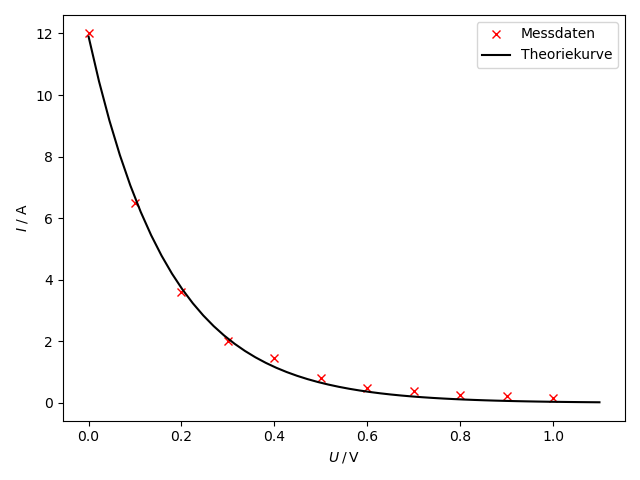
\includegraphics[height=80mm]{bilder/An1.png}
    \caption{Das Anlaufgebiet bei maximaler Heizleistung.\label{Abbildung12} }
\end{figure}

\begin{align}
    \intertext{Aus der Ausgleichsrechnung ergibt sich für die Parameter}
    \text{a} = ( 11,89 \pm 0,16 )\,\unit{\nano\ampere}\,, \notag\\
    \text{b} = ( 2000,51 \pm 50,86 )\,.\notag
    \intertext{Die Temperatur T ist dabei der Parameter b mit}
    \text{T} = ( 2000,51 \pm 50,86 )\,\,\unit{\kelvin}.\notag
\end{align}

\subsection{Kathodentemperatur aus den verschiedenen Heizleistungen}

\begin{align}
    \intertext{Die Kathodentemperatur T wird aus der Leistungsbilanz des Heizstromfadens gewonnen. 
    Dazu beträgt die Leistung:}
    \text{N}_{\text{zu}} = \text{U}_{\text{Heiz}} \cdot \text{I}_{\text{Heiz}}\,.\notag
    \intertext{Die Wärmestrahlung und Wärmeleitung wird dabei abgegeben. 
    Angenommen wird der Wert für die Wärmeleitung einen Wert von $\text{N}_{\text{w}} = 1\,\unit{\watt}$. 
    Die Strahlungsleistung ergibt sich nach dem Stefan-Boltzmannschen Gesetz zu}
    \text{N}_{\text{zu}} = \text{f} \cdot \eta \cdot \sigma \cdot \text{T}^{4}\,.\notag
    \intertext{Hierbei beträgt die Stefan-Boltzmannsche Strahlungskonstant $\sigma = 5,7 \cdot 10^{-12}\,\frac{\unit{\watt}}{\unit{\centi\meter}^{2}\, \text{K}^{4}}$, die Kantenoberfläche $\text{f} = 0,35\,\unit{\centi\meter}^{2}$ und der Emissionsgrad $\eta = 0,28$. 
    Aus dem Energiesatz folgt}
    \text{N}_{\text{zu}} = \text{N}_{\text{Str}} + \text{N}_{\text{WL}} \notag\\
    \iff \text{U}_{\text{Heiz}} \cdot \text{I}_{\text{Heiz}} = \text{f} \cdot \eta \cdot \sigma \cdot \text{T}^{4} + \text{N}_{\text{WL}\,. \label{5}}
    \intertext{Die berechneten Temperaturen folgen durch die Umstellung der Gleichung (\ref{5}) und werden ebenso in der Tabelle \ref{Tabelle4} festgehalten.} \notag
\end{align}

\begin{table}[H]
    \centering
    \caption{Die Kathodentemperatur T} 
    \label{Tabelle4}
    \begin{tabular} {c  c  c}
        \toprule
        {$ \text{U}_{\text{Heiz}} \mathbin{/} \unit{\volt} $} &
        {$ \text{I}_{\text{Heiz}} \mathbin{/} \unit{\ampere}$} &
        {$ \text{T} \mathbin{/} \unit{\kelvin}$} \\
        \midrule
        5   & 2,0 & 2003,48 \\
        5   & 2,1 & 2030,75 \\
        5,5 & 2,2 & 2111,33 \\
        6   & 2,3 & 2187,90 \\
        6,2 & 2,4 & 2232,66 \\
        7   & 2,5 & 2331,29 \\
        \bottomrule
    \end{tabular} 
\end{table}

\subsection{Austrittarbeit des Kathodenmaterials}

\begin{align*}
    \intertext{Die Austrittsarbeit wird aus den T- und den zugehörigen Is-Werten hergeleitet.
    Die Richardson-Gleichung (\ref{4}) wird nach $\phi$ umgestellt zu:} 
    \text{W}_{\text{A}} = e_{0} \cdot \phi = -\text{T} \,\text{k}_{\text{B}} \cdot \ln \left( \frac{\text{j}_{\text{s}}\,\text{h}^{3}}{4\,\pi\,e_{0}\cdot \text{m}_{0}\,\text{k}^{2}_{\text{B}}\,\text{T}^{4} } \right) \,,
    \intertext{mit}
    \text{j}_{s} = \frac{\text{I}_{\text{s}}}{\text{f}}\,.
    \intertext{Somit ergibt sich die Austrittsarbeit von Wolfram für die sechs Kennlinien:}
\end{align*} 

\begin{table}[H]
    \centering
    \caption{} 
    \label{Tabelle}
    \begin{tabular} {c  c  c  c}
        \toprule
        {Kennlinien} &
        {$ \text{W}_{\text{A}} \mathbin{/} \cdot 10^{-19}\,\text{J} $} &
        {$ \text{W}_{\text{A}} \mathbin{/} \text{eV} $} \\
        \midrule
        1 & 9,173 & 5,72 \\
        2 & 9,100 & 5,68 \\
        3 & 9,211 & 5,74 \\
        4 & 9,486 & 5,92 \\
        5 & 9,536 & 5,95 \\
        6 & 9,954 & 6,21 \\
        \bottomrule
    \end{tabular} 
\end{table}

\begin{align*}
    \intertext{Die Austrittsarbeit von Wolfram beträgt}
    \overline{\text{W}}_{\text{A}} = ( 5,87 \pm 0,18 )\,\text{eV}\,.
\end{align*}